\documentclass[a4paper,UTF8]{article}
\usepackage{ctex}
\usepackage[margin=1.25in]{geometry}
\usepackage{color}
\usepackage{graphicx}
\usepackage{amssymb}
\usepackage{amsmath}
\usepackage{amsthm}
\usepackage{enumerate}
\usepackage{bm}
\usepackage{hyperref}
\usepackage{epsfig}
\usepackage{color}
\usepackage{mdframed}
\usepackage{lipsum}
\usepackage{graphicx}
\usepackage{tikz}
\newmdtheoremenv{thm-box}{Theorem}
\newmdtheoremenv{prop-box}{Proposition}
\newmdtheoremenv{def-box}{定义}

\usepackage{listings}
\usepackage{xcolor}
\lstset{
	numbers=left, 
	numberstyle= \tiny, 
	keywordstyle= \color{ blue!70},
	commentstyle= \color{red!50!green!50!blue!50}, 
	frame=shadowbox, % 阴影效果
	rulesepcolor= \color{ red!20!green!20!blue!20} ,
	escapeinside=``, % 英文分号中可写入中文
	xleftmargin=2em,xrightmargin=2em, aboveskip=1em,
	framexleftmargin=2em
} 

\usepackage{booktabs}

\setlength{\evensidemargin}{.25in}
\setlength{\textwidth}{6in}
\setlength{\topmargin}{-0.5in}
\setlength{\topmargin}{-0.5in}
% \setlength{\textheight}{9.5in}
%%%%%%%%%%%%%%%%%%此处用于设置页眉页脚%%%%%%%%%%%%%%%%%%
\usepackage{fancyhdr}                                
\usepackage{lastpage}                                           
\usepackage{layout}                                             
\footskip = 10pt 
\pagestyle{fancy}                    % 设置页眉                 
\lhead{2018年春季}                    
\chead{机器学习导论}                                                
% \rhead{第\thepage/\pageref{LastPage}页} 
\rhead{作业三}                                                                                               
\cfoot{\thepage}                                                
\renewcommand{\headrulewidth}{1pt}  			%页眉线宽,设为0可以去页眉线
\setlength{\skip\footins}{0.5cm}    			%脚注与正文的距离           
\renewcommand{\footrulewidth}{0pt}  			%页脚线宽,设为0可以去页脚线

\makeatletter 									%设置双线页眉                                        
\def\headrule{{\if@fancyplain\let\headrulewidth\plainheadrulewidth\fi%
\hrule\@height 1.0pt \@width\headwidth\vskip1pt	%上面线为1pt粗  
\hrule\@height 0.5pt\@width\headwidth  			%下面0.5pt粗            
\vskip-2\headrulewidth\vskip-1pt}      			%两条线的距离1pt        
 \vspace{6mm}}     								%双线与下面正文之间的垂直间距              
\makeatother  

%%%%%%%%%%%%%%%%%%%%%%%%%%%%%%%%%%%%%%%%%%%%%%
\numberwithin{equation}{section}
%\usepackage[thmmarks, amsmath, thref]{ntheorem}
\newtheorem{theorem}{Theorem}
\newtheorem*{definition}{Definition}
\newtheorem*{solution}{Solution}
\newtheorem*{prove}{Proof}
\newcommand{\indep}{\rotatebox[origin=c]{90}{$\models$}}

\usepackage{multirow}

%--

\tikzset{
	treenode/.style = {shape=rectangle, rounded corners,
		draw, align=center,
		top color=white, bottom color=blue!20},
	root/.style     = {treenode, font=\Large, bottom color=red!30},
	env/.style      = {treenode, font=\ttfamily\normalsize},
	dummy/.style    = {circle,draw}
}

%--
\begin{document}
\title{机器学习导论\\
作业三}
\author{学号, 作者姓名, 邮箱}
\maketitle



\section{[15pts] Decision Tree I}

\begin{enumerate}[ {(}1{)}]
	\item \textbf{[5pts]} 假设一个包含三个布尔属性${X, Y, Z}$的空间,并且目标函数是$f(x,y,z) = x\ \mathbf{XOR}\ z$,其中$\mathbf{XOR}$为异或运算符。令$H$为基于这三个属性的决策树,请问:目标函数$f$可实现吗?如果可实现,画出相应的决策树以证明;如果不可实现,请论证原因;
	
	\item \textbf{[10pts]} 现有如表~\ref{table:ranking}所示数据集:
	
	\begin{table}[!h]
		\centering
		\caption{样例表} \vspace{2mm}\label{table:ranking}
		\begin{tabular}{c c c|c}\hline
			$X$ & $Y$ & $Z$ & $f$ \\
			\hline
			$1$ & $0$  & $1$ &  $1$\\
			$1$ & $1$  & $0$ &  $0$\\
			$0$ & $0$  & $0$ &  $0$\\
			$0$ & $1$  & $1$ &  $1$\\
			$1$ & $0$  & $1$ &  $1$\\
			$0$ & $0$  & $1$ &  $0$\\
			$0$ & $1$  & $1$ &  $1$\\
			$1$ & $1$  & $1$ &  $0$\\
			\hline
		\end{tabular}
	\end{table}
	
	请画出由该数据集生成的决策树。划分属性时要求以信息增益 (information gain)为准则。当信息增益 (information gain)相同时,依据字母顺序选择属性即可。
\end{enumerate}
\begin{solution}
~\\
~\\
~\\
~\\
~\\
~\\
\begin{enumerate}
\item[(1)]目标函数$f$是可以实现的,决策树如下所示:\\\\
\begin{tikzpicture}
[
grow                    = down,
edge from parent/.style = {draw, -latex},
every node/.style       = {font=\footnotesize}
]
\tikzstyle{level 1}=[level distance=20mm,sibling distance=5cm]
\tikzstyle{level 2}=[level distance=20mm,sibling distance=2cm]
\tikzstyle{level 3}=[level distance=20mm,sibling distance=1cm]
\node [root] {x = ?}
child { node [env] {z = ?}
    child { node [env] { f = 0}
        edge from parent node [below] {0} }
    child { node [env] {f = 1}
        edge from parent node [below] {1} }
	edge from parent node [below] {0} }
child { node [env] {z = ?}
    child { node [env] { f = 1}
        edge from parent node [below] {0} }
    child { node [env] {f = 0}
        edge from parent node [below] {1} }
	edge from parent node [below] {1} };
\end{tikzpicture}\\
\item[(2)]
按照信息增益为准则,划分依据为:\\
第一层根结点:\\
如果选择$X$划分:
\begin{equation}
\begin{aligned}
Gain(D, X) =& Ent(D) - \sum_{v=1}^{2}\frac{|D^v|}{|D|}Ent(D^v) \\
=& 1 - 1 = 0 
\end{aligned}
\end{equation}
如果选择$Y$划分:
\begin{equation}
Gain(D, Y) = 1 - 1 = 0 
\end{equation}
如果选择$Z$划分:
\begin{equation}
Gain(D, Y) = 1 - \frac{3}{4}\times 0.918 = 0.6885 
\end{equation}
所以选择$Z$划分。\\
第二层第一个结点都是同一类,现在考虑第二个结点的划分:\\
如果选择$X$划分:
\begin{equation}
Gain(D, X) = 0.918 - 0.918 = 0
\end{equation}
如果选择$Y$划分:
\begin{equation}
Gain(D, Y)  = 0.918 - 0.918 = 0
\end{equation}
所以按照字母顺序选择$X$划分。\\
根据数据集生成的决策树如下:\\\\
\begin{tikzpicture}
[
grow                    = down,
edge from parent/.style = {draw, -latex},
every node/.style       = {font=\footnotesize}
]
\tikzstyle{level 1}=[level distance=20mm,sibling distance=9cm]
\tikzstyle{level 2}=[level distance=20mm,sibling distance=4cm]
\tikzstyle{level 3}=[level distance=20mm,sibling distance=2cm]
\node [root] {Z = ?}
child { node [env] {f = 0}
	edge from parent node [below] {0} }
child { node [env] {X = ?}
	child { node [env] { Y = ?}
		child {node [env] {f=0}
			edge from parent node [below] {0} }
		child {node [env] {f=1}
			edge from parent node [below] {1} }
		edge from parent node [below] {0} }
	child { node [env] { Y = ?}
		child {node [env] {f=1}
			edge from parent node [below] {0} }
		child {node [env] {f=0}
			edge from parent node [below] {1} }
		edge from parent node [below] {1} }
	edge from parent node [below] {1} };
\end{tikzpicture}\\
\end{enumerate}
\end{solution}
\newpage



 \section{[20pts] Decision Tree II}
 考虑如下矩阵:
 $$
 \begin{bmatrix}
 4 & 6 & 9 & 1 & 7 & 5 \\
 1 & 6 & 5 & 2 & 3 & 4
 \end{bmatrix}^T
 $$

 该矩阵代表了$6$个样本数据,每个样本都包含$2$个特征$f_1$和$f_2$。这$6$个样本数据对应的标签如下:
 $$
 \begin{bmatrix}
 1 & 0 & 1 & 0 & 1 & 0
 \end{bmatrix}^T
 $$

 在这个问题中,我们要构造一个深度为$2$的树进行分类任务。

 \begin{enumerate}[ {(}1{)}]
 	\item \textbf{[5pts]} 请计算根结点 (root) 的熵值 (entropy);

 	\item \textbf{[10pts]} 请给出第一次划分的规则,例如$f_1 \geq 4, f_2 \geq 3$。对于第一次划分后产生的两个结点,请给出下一次划分的规则;

 	提示:可以直观判断,不必计算熵。

 	\item \textbf{[5pts]} 现在回到根结点 (root),并且假设我们是建树的新手。是否存在一种划分使得根结点 (root) 的信息增益 (information gain) 为$0$?
 \end{enumerate}

 \begin{solution}
 ~\\
 \begin{enumerate}
 \item [(1)]
 根结点的熵值为
 \begin{equation}
 Ent(D) = -(\frac{3}{6}\log_2\frac{3}{6} + \frac{3}{6}\log_2\frac{3}{6}) = 1.000
 \end{equation}
 \item [(2)]
 规则如图1所示。第一次划分的规则为$f_1\leq 6$。不满足$f_1\leq 6$的结点的所有样本的标签都是$1$,所以这一部分不需要再次划分。第一次划分之后,满足$f_1\leq 6$的节点的第二次划分的规则为$f_2\leq 1$,其中满足$f_2\leq 1$的结点的样本的标签都都是$1$,不满足的都是$0$,所以不需要再次划分。
 \begin{figure}[!h]
 	\centering   
 	\includegraphics[scale=0.5]{coordinate1.png}  
 	\caption{划分规则} 
 	\label{coordinate1}
 \end{figure}
 \item [(3)]
 规则如图2所示。按照$f_2\leq 2$来划分,将$D$分成了$D^1$和$D^2$两个部分。其中$D^1$包含第一个和第四个样例。由此可得
 \begin{equation}
 Ent(D^1) =  -(\frac{1}{2}\log_2\frac{1}{2} + \frac{1}{2}\log_2\frac{1}{2}) = 1.000
 \end{equation}
 \begin{equation}
 Ent(D^2) = -(\frac{2}{4}\log_2\frac{2}{4} + \frac{2}{4}\log_2\frac{2}{4}) = 1.000
 \end{equation}
 所以可得信息增益为
 \begin{equation}
 \begin{aligned}
 Gain(D, f_2\leq 2) &= Ent(D) - \sum_{v=1}^{2}\frac{|D^v|}{|D|}Ent(D^v)\\
 &= 1 - (\frac{2}{6}\times 1 + \frac{4}{6}\times 1)\\
 &= 0
 \end{aligned}
 \end{equation}
 \begin{figure}[!h]
 	\centering   
 	\includegraphics[scale=0.5]{coordinate2.png}  
 	\caption{划分规则} 
 	\label{coordinate2}
 \end{figure}
 \end{enumerate}
 \end{solution}
\newpage

 \section{[25pts] Universal Approximator}
 已知函数$f:[-1, 1]^n \mapsto [-1, 1]$满足$\rho$-Lipschiz性质。 给定误差$\epsilon > 0$,请构造一个激活函数为\mbox{ sgn($\mathbf{x}$) }的神经网络$ \mathcal{N}:[-1,1]^n \mapsto [-1,1] $,使得对于任意的输入样本$ \mathbf{x} \in [-1,1]^n $,有$|f(\mathbf{x}) - \mathcal{N}(\mathbf{x})| \leq \epsilon$。\\
 (Lipschiz条件为:$ \forall \mathbf{x}, \mathbf{y} \in [-1,1]^n$,$ \exists \rho > 0$,$ \mbox{ s.t. } |f(\mathbf{x})-f(\mathbf{y})| \leq \rho \lVert \mathbf{x} - \mathbf{y} \rVert_2 $,其中\mbox{ sgn($\mathbf{x}$) }的定义参见《机器学习》第98页。)
 
  \begin{enumerate}[ {(}1{)}]
 	\item \textbf{[5pts]} 请画出构造的神经网络$\mathcal{N}$的示意图;
 	
 	\item \textbf{[10pts]} 请对构造的神经网络进行简要的说明(写清每一层的线性组合形式,也就是结点间的连接方式和对应的权重);
 	
 	\item \textbf{[10pts]} 证明自己构造的神经网络的拟合误差满足要求。
 \end{enumerate}


 \begin{solution}
	此处用于写解答(中英文均可)
 \end{solution}
\newpage

\section{[40pts] Neural Network in Practice}
通过《机器学习》课本第5章的学习,相信大家已经对神经网络有了初步的理解。深度神经网络在某些现实机器学习问题,如图像、自然语言处理等表现优异。本次作业旨在引导大家学习使用一种深度神经网络工具,快速搭建、训练深度神经网络,完成分类任务。

我们选取PyTorch为本次实验的深度神经网络工具,有了基础工具,我们就能如同搭积木一样构建深度神经网络。\href{http://pytorch.org/}{PyTorch}是Facebook开发的一种开源深度学习框架,有安装方便、文档齐全、构架方便、训练效率高等特点。本次作业的首要任务就是安装PyTorch。

目前PyTorch仅支持Linux和MacOS操作系统,所以Window用户需要装一个Linux虚拟机或者直接安装Linux系统。PyTorch安装很方便,只需要在其主页中的Get Start一栏选择对应的环境设置,便能够一键安装。有GPU的同学也可以尝试安装GPU版本的PyTorch。为保证此次作业的公平性,只要求使用CPU进行网络训练,当然有条件的同学也可以尝试使用GPU进行训练。在批改作业时,助教会提供Python 2.7、3.5、3.6三种环境进行实验验证。

我们选取CIFAR10作为本次作业的训练任务。\href{https://en.wikipedia.org/wiki/CIFAR-10}{CIFAR10}是一个经典的图片分类数据集,数据集中总共有60000张32$\times$32的彩色图片,总共有10类,每类6000张图片,其中50000张图片构成训练集,10000张图片构成测试集。PyTorch通过torchvision给用户提供了获取CIFAR10的方法,详细信息可见\href{http://pytorch.org/tutorials/beginner/blitz/cifar10_tutorial.html}{PyTorch的教程}。此外关于CIFAR10分类准确率排行可见此\href{http://rodrigob.github.io/are_we_there_yet/build/classification_datasets_results.html}{链接}。

下面我们将尝试使用PyTorch来解决实际问题:

\begin{enumerate}[(1)]
	\item \textbf{[15pts]} 首先我们跟随PyTorch的教程,用一个简单的卷积神经网络(Convolutional Neural Network, CNN),完成CIFAR10上的分类任务,具体要求如下:
	
	\begin{itemize}
		\item \textbf{[7pts]} 在代码实现之前,大家可能需要对CNN网络进行一定的了解,请大家自行查阅资料(PyTorch的教程中也有部分介绍CNN网络),并在实验报告中给出对CNN的见解:主要回答什么是卷积层,什么是Pooling层,以及两者的作用分别是什么;
		\item \textbf{[8pts]} 接下来就是具体的代码实现和训练。教程会手把手教你完成一次训练过程,其中使用SGD作为优化方法,请同学们自行调整epoch的大小和学习率,完成此次训练。另外,请在实验报告中给出必要的参数设置,以及训练结果如最终的loss、在测试集上的准确率等;
	\end{itemize}
	\item \textbf{[20pts]} 显然,这样一个简单的网络在CIFAR10上并不能取得令人满意的结果,我们需要选取一个更为复杂的网络来提升训练效果。在此小题中,我们选取了CIFAR10准确率排行榜上排名第二的结构,具体参见\href{https://arxiv.org/pdf/1412.6806.pdf}{论文链接}。为了方便大家实现,我们直接给出了网络结构如图\ref{network_structure}所示。请大家搭建完成此网络结构,并选择Adam为优化器,自行调整相关参数完成训练和预测,实验结果报告内容同第(1)小题;
	\begin{figure}[!h]
		\centering   
		\includegraphics[width=0.99\textwidth, height=0.15\textwidth]{nn_structure.png}  
		\caption{待实现网络结构} 
		\label{network_structure}
	\end{figure}
	\item \textbf{[5pts]} 通过上一题实验我们可以发现,即使使用现成的网络结构也不一定能达到与其相同的训练效果。请大家分析其中的原因,并谈谈本次实验的感想,以及对深度学习调参的体会。
\end{enumerate}

\noindent{\textbf{实验报告.}}

\begin{enumerate}
\item [(1)]
~\\
\textbf{对CNN的见解}:卷积神经网络是一种非常强大的,适合用于图像,视频识别以及自然语言处理的神经网络的。卷积神经网络本身就是一种特殊的神经网络,其训练的流程为:输入层接受训练集数据,通过隐层一层层传递到输出层,输出与真实标签进行比较,得到损失函数,然后再通过反向传播来调整隐层的参数,进而降低损失函数,来使得预测结果逼近与真实标签。CNN中比较特殊的隐层结构是卷积层和pooling层,其中卷积层主要承担了对特定模式的识别工作,pooling层主要起到了采样的作用。\\
\textbf{卷积层的概念}:是卷积神经网络的核心,承担了卷积神经网络大部分的工作量。\\
\textbf{卷积层的作用}:卷积层的作用主要在于提取特征,这个操作类似于信号处理中的滤波,和人类大脑认知世界也有几分相似。这个操作的实现用到了卷积的方法。具体的,如果输入的数据大小为$H\times W\times D$(此处先假设batch size为1,其中D表示channel数量),那么卷积层就会有诸多大小为$H'\times W'\times D$的filter(其中$H' < H$而且$W' < W$)。通过将一个filter“覆盖”在输入数据上,会得到输入数据上的一个和filter相同大小的数据块,把数据块和filter对应位置的元素相乘然后求和,可以得到一个标量值,把filter“覆盖”到数据的不同位置可以得到很多标量值,将这些标量值按照顺序排列起来可以得到一个activation map,每一个filter针对每一个输入数据都会得到一个activation map,把多个filter对应的activation map堆叠在一起就可以得到下一个隐层的输入数据。每一个卷积层得到的activation map其实就是对某种特征的提取,如果map中某个元素值很大,就说明这个元素对应的输入数据的特定位置有可能存在某种特征。所以activation map实际上可以反应出特征在输入数据集中的分布。卷积层可以识别的特征多种多样的,一般第一卷积层只能识别一些简单的特征,例如边缘,曲线,角,更多层的卷积层可以识别到更加复杂的特征。\\
\textbf{Pooling层的概念}:pooling层也是卷积神经网络中一个重要的结构,他的主要功能在于对数据进行采样。\\
\textbf{Pooling层的作用}:总体来讲pooling层的作用在于减少数据大小,减少参数,降低运算量,减低训练时间,防止过拟合,提高泛化能力,同时还可以保持特征的不变形(包括平移,旋转,尺度等方面)。具体的,pooling层就是按照一定的比例对输入数据进行采样,常见的有max-pooling和average-pooling。常见的做法是将数据分成$2\times 2$的数据块然后从每个数据块中选择一个最大值(或者平均值)来代替整个数据块。其中max-pooling采样操作还能够保持输入数据的特征不变型,比如说某个数据块中出现了某个特征,反映在输入数据上就是某个元素的值非常大。当我们在对这个数据块采样的时候,为了在下一层维持这个特征的表现,我们选择了最大的数值作为采样后的结果,这背后蕴含了即便数据缩小了,我们仍然尽可能保持原有的特征这一思想,所以实践中往往max-pooling表现会比较好。实践中会在卷积层之间周期性的插入pooling层来提升整体的效果。
	
\item [(2)]
~\\
	
\end{enumerate}

\end{document}